%-----------------------------------------------------------------------------------------------------------------------------------------------%
%	The MIT License (MIT)
%
%	Copyright (c) 2021 Jitin Nair
%
%	Permission is hereby granted, free of charge, to any person obtaining a copy
%	of this software and associated documentation files (the "Software"), to deal
%	in the Software without restriction, including without limitation the rights
%	to use, copy, modify, merge, publish, distribute, sublicense, and/or sell
%	copies of the Software, and to permit persons to whom the Software is
%	furnished to do so, subject to the following conditions:
%	
%	THE SOFTWARE IS PROVIDED "AS IS", WITHOUT WARRANTY OF ANY KIND, EXPRESS OR
%	IMPLIED, INCLUDING BUT NOT LIMITED TO THE WARRANTIES OF MERCHANTABILITY,
%	FITNESS FOR A PARTICULAR PURPOSE AND NONINFRINGEMENT. IN NO EVENT SHALL THE
%	AUTHORS OR COPYRIGHT HOLDERS BE LIABLE FOR ANY CLAIM, DAMAGES OR OTHER
%	LIABILITY, WHETHER IN AN ACTION OF CONTRACT, TORT OR OTHERWISE, ARISING FROM,
%	OUT OF OR IN CONNECTION WITH THE SOFTWARE OR THE USE OR OTHER DEALINGS IN
%	THE SOFTWARE.
%	
%
%-----------------------------------------------------------------------------------------------------------------------------------------------%

%----------------------------------------------------------------------------------------
%	DOCUMENT DEFINITION
%----------------------------------------------------------------------------------------

% article class because we want to fully customize the page and not use a cv template
\documentclass[a4paper,12pt]{article}

%----------------------------------------------------------------------------------------
%	FONT
%----------------------------------------------------------------------------------------

% % fontspec allows you to use TTF/OTF fonts directly
% \usepackage{fontspec}
% \defaultfontfeatures{Ligatures=TeX}

% % modified for ShareLaTeX use
% \setmainfont[
% SmallCapsFont = Fontin-SmallCaps.otf,
% BoldFont = Fontin-Bold.otf,
% ItalicFont = Fontin-Italic.otf
% ]
% {Fontin.otf}

%----------------------------------------------------------------------------------------
%	PACKAGES
%----------------------------------------------------------------------------------------
\usepackage{url}
\usepackage{parskip} 
%\usepackage[english]{babel}
\usepackage{csquotes}

%other packages for formatting
\RequirePackage{color}
\RequirePackage{graphicx}
\usepackage[dvipsnames]{xcolor}
\usepackage[left=1.5cm,top=1.5cm,right=1.5cm,bottom=1.9cm,nofoot]{geometry}

%tabularx environment
\usepackage{tabularx}
\usepackage{booktabs}

%for lists within experience section
\usepackage{enumitem}

% centered version of 'X' col. type
\newcolumntype{C}{>{\centering\arraybackslash}X} 

%to prevent spillover of tabular into next pages
\usepackage{supertabular}
\usepackage{tabularx}
\newlength{\fullcollw}
\setlength{\fullcollw}{0.47\textwidth}

%custom \section
\usepackage{titlesec}				
\usepackage{multicol}
\usepackage{multirow}
\usepackage{tikz}
\usepackage{tikzpagenodes}
\usepackage{bm}
\usepackage{array, makecell}
\renewcommand\theadfont{\bfseries}
\usetikzlibrary{calc}
\usetikzlibrary{shapes.geometric}
\usetikzlibrary{decorations.pathmorphing}

%CV Sections inspired by: 
%http://stefano.italians.nl/archives/26
\titleformat{\section}{\Large\scshape\raggedright}{}{0em}{}[\titlerule]
\titlespacing{\section}{0pt}{10pt}{10pt}

%%%%%
%for publications
\usepackage[backend=biber, style=numeric, sorting=none]{biblatex}

%Setup hyperref package, and colours for links
\usepackage[unicode, draft=false]{hyperref}
\definecolor{linkcolour}{rgb}{0,0.2,0.6}
\hypersetup{colorlinks,breaklinks,urlcolor=linkcolour,linkcolor=linkcolour}
\addbibresource{citations.bib}
% Use the note field as the citation label and remove brackets
\DeclareFieldFormat{labelnumber}{\textbf{\thefield{note}}}
\renewcommand*{\labelalphaothers}{}

% Ensure numeric labels are cleared
\AtEveryBibitem{
  \clearfield{labelnumber}
}
%\setlength\bibitemsep{1em}
%%%%%

%for social icons
\usepackage{fontawesome5}
\usepackage{fancyhdr}

% remove word-splits
\usepackage[none]{hyphenat}

\newcommand\rating[2]{%
  \pgfmathsetmacro\pgfxa{#1 + 1}%
  \tikzstyle{scorestars}=[star, star points=5, star point ratio=2.25, draw, inner sep=0.15em, anchor=outer point 3]%
  \begin{tikzpicture}[baseline]
    \foreach \i in {1, ..., #2} {
      \pgfmathparse{\i<=#1 ? "black" : "white"}
      \edef\starcolor{\pgfmathresult}
      \draw (\i*1.3em, 0) node[name=star\i, scorestars, fill=\starcolor]  {};
    }
    \pgfmathparse{#1>int(#1) ? int(#1+1) : 0}
    \let\partstar=\pgfmathresult
    \ifnum\partstar>0
      \pgfmathsetmacro\starpart{#1-(int(#1))}
      \path [clip] ($(star\partstar.outer point 3)!(star\partstar.outer point 2)!(star\partstar.outer point 4)$) rectangle 
      ($(star\partstar.outer point 2 |- star\partstar.outer point 1)!\starpart!(star\partstar.outer point 1 -| star\partstar.outer point 5)$);
      \fill (\partstar*1em, 0) node[scorestars, fill=yellow]  {};
    \fi
  \end{tikzpicture}%
}

%----------------------------------------------------------------------------------------
%	BEGIN DOCUMENT
%----------------------------------------------------------------------------------------
\begin{document}
% non-numbered pages
\pagestyle{fancy}
\fancyhf{} % sets both header and footer to nothing
\renewcommand{\headrulewidth}{0pt}
%----------------------------------------------------------------------------------------
%	TITLE
%----------------------------------------------------------------------------------------

% \begin{tabularx}{\linewidth}{ @{}X X@{} }
% \huge{Your Name}\vspace{2pt} & \hfill \emoji{incoming-envelope} email@email.com \\
% \raisebox{-0.05\height}\faGithub\ username \ | \
% \raisebox{-0.00\height}\faLinkedin\ username \ | \ \raisebox{-0.05\height}\faGlobe \ mysite.com  & \hfill \emoji{calling} number
% \end{tabularx}

% {\Huge \textbf{Curriculum Vitae \\[0.3cm]}} 
% {\Large \textit{Oscar Stommendal}} \\[-0.7cm]
{\Huge \textbf{Curriculum Vitae} \hfill \textit{Oscar Stommendal}} \\[-0.7cm]

\hrulefill%{11.9cm}{0.4pt} \\[-0.6cm]

\textsc{BSc Engineering Physics $\vert$ MSc Physics $\vert$ BSc Business and Economics \\[0.2cm] Chalmers $\vert$ NTU Singapore $\vert$ University of Gothenburg}\\[-0.9cm]

\hrulefill%{11.9cm}{0.4pt}

\begin{tabular}[c]{l|c|c|c|c}
    \href{mailto:oscar.stommendal01@gmail.com}{\raisebox{-0.05\height}\faEnvelope \ Email \hspace{0.05cm}}& \hspace{0.1cm}
    \href{https://linkedin.com/in/oscar-stommendal} {\raisebox{-0.05\height}\faLinkedin\ LinkedIn \hspace{0.05cm}} & \hspace{0.25cm}%\href{tel:+46706617353}{\raisebox{-0.05\height}\faMobile \ iPhone} &
    \href{https://github.com/stommen} {\raisebox{-0.05\height}\faGithub \ Github \hspace{0.05cm}} & \hspace{0.15cm}
    \href{https://stommen.github.io}{\raisebox{-0.05\height}\faGlobe \ Personal Webpage} \hspace{0.05cm} & \hspace{-0.15cm}
    \hspace{0.15cm} \href{https://www.google.com/maps/place/Göteborg,+Sverige/@57.7005638,11.5642129,10z/data=!3m1!4b1!4m6!3m5!1s0x464f8e67966c073f:0x4019078290e7c40!8m2!3d57.70887!4d11.97456!16zL20vMDM0M18?entry=ttu&g_ep=EgoyMDI1MDEyOS4xIKXMDSoASAFQAw%3D%3D}{\raisebox{-0.05\height}\faMapMarker \ Gothenburg}
\end{tabular}
\hfill
% \begin{tikzpicture}[remember picture,overlay]
% \clip ($(current page text area.north east)!0.10!(current page text area.south east)!0.12!(current page text area.north west)$)
%   circle (2.2cm) node {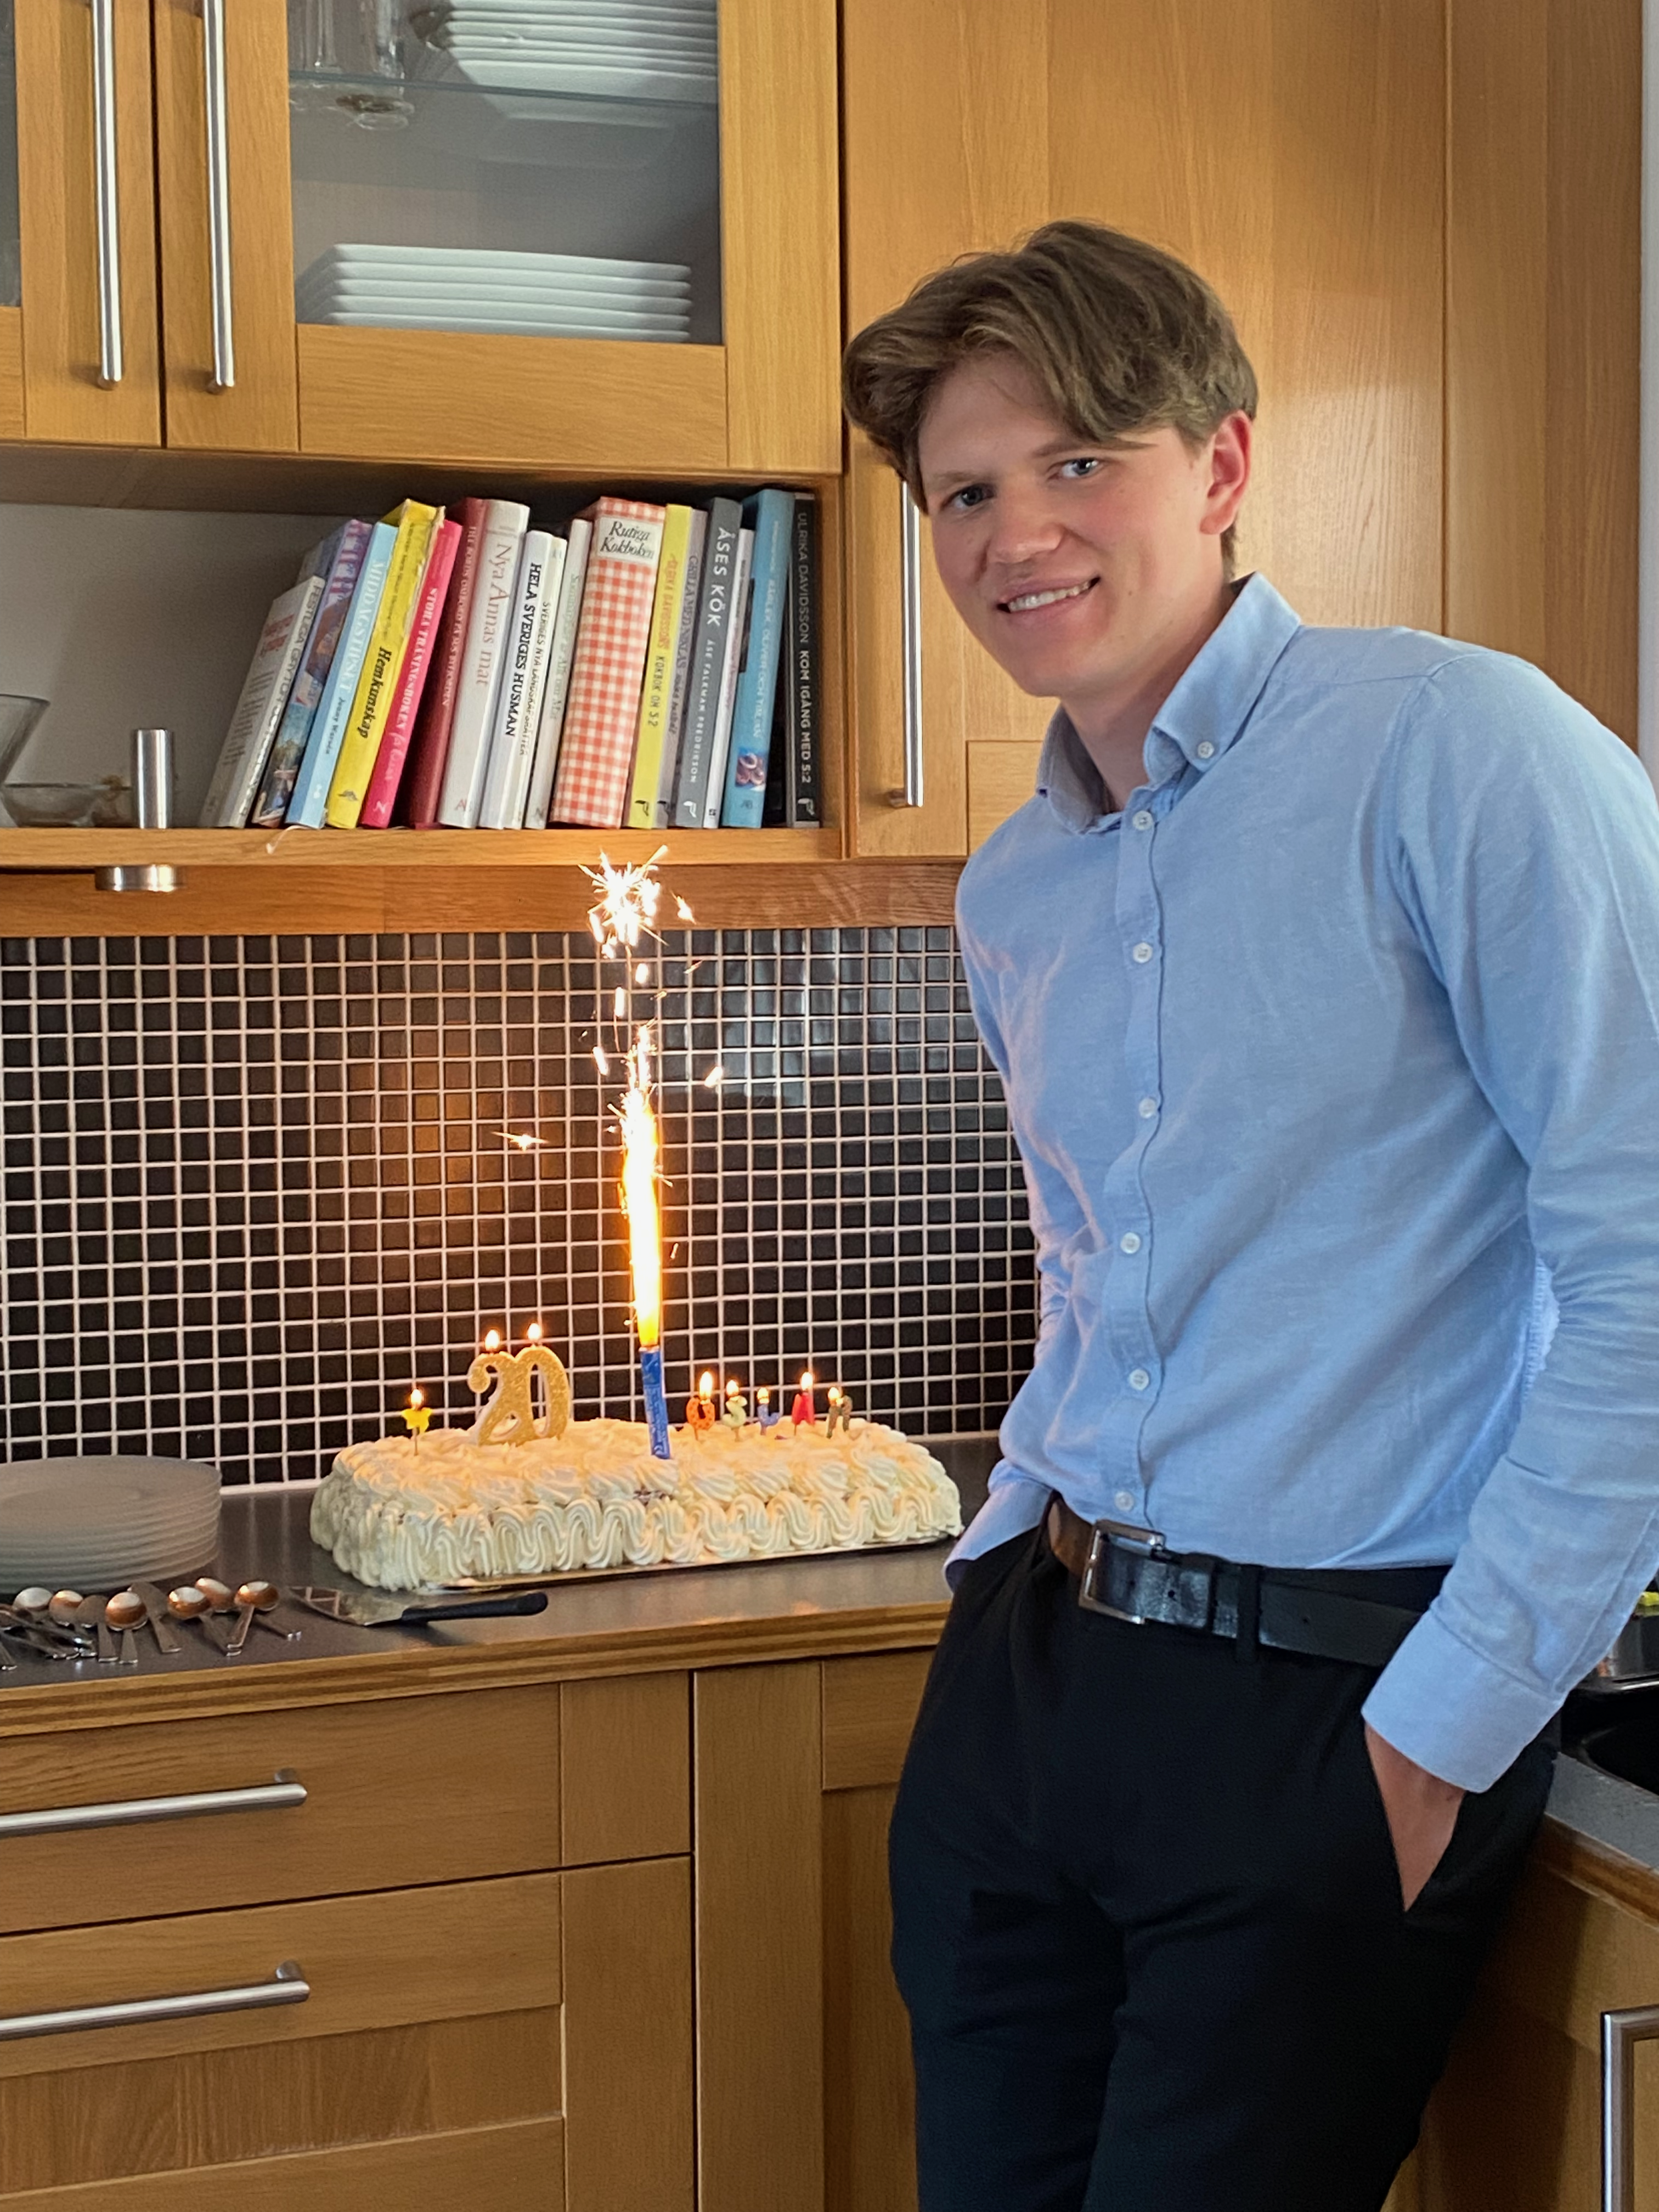
\includegraphics[width=4.5cm]{photos/cv_bild.pdf}};
% \end{tikzpicture}
\hspace*{0.1cm}\\[-0.3cm]
%\begin{tabularx}{\linewidth}{@{} C @{}}
%\Huge{Oscar Stommendal} \\[7.5pt]
%\href{https://linkedin.com/in/oscarstommendal}{\raisebox{-0.05\height}\faLinkedin\ oscarstommendal} \ $|$ \ 
%\href{mailto:oscar.stommendal01@gmail.com}{\raisebox{-0.05\height}\faEnvelope \ oscar.stommendal01@gmail.com} \ $|$ \ 
%href{tel:+46706617353}{\raisebox{-0.05\height}\faMobile \ +46 70-661-7353} \\
%\end{tabularx}
%----------------------------------------------------------------------------------------
% EXPERIENCE SECTIONS
%----------------------------------------------------------------------------------------
%Interests/ Keywords/ Summary
\section{Goal with Application}
%Through the CERN Summer Student Programme, I aim to deepen my understanding of science and technology while gaining experience in a world-class research environment. This opportunity will help me advance toward a future career at the forefront of technological advancements by collaborating with leading researcher and connecting with like-minded peers from around the world.
%Through a summer internship at Novatron, I hope to kick-start my career in the fusion- and renewable energy sector. I am eager to apply my knowledge in physics and engineering to real-world problems, and to learn from experienced professionals in the field. I am confident that my analytical skills, problem-solving abilities and positive attitude will make me a valuable addition to the team.
%At Ericsson, I hope to gain valuable experience and develop my engineering skills. I am eager to apply my knowledge in physics and engineering to real-world problems, and to learn from experienced professionals in the field. I am confident that my analytical skills, problem-solving abilities and positive attitude will make me a valuable addition to the team.
%At Nasdaq, I am very excited to apply my knowledge in physics, engineering and economics to solve real-world problems. I hope that the internship will provide me with valuable experience for a future career in the forefront of technological advancements at global-leading companies. I am confident that my skills and positive attitude will be a valuable addition to the team.
%At Spotify, I aim to merge my passion for music with my skills in physics, engineering, and economics to tackle real-world challenges. I am excited to learn from experienced professionals and gain valuable experience for a future career at globally leading companies, where I aspire to drive technological advancements and shape the future. With strong analytical skills, a problem-solving mindset, and a positive attitude, I am confident in my ability to contribute meaningfully to the team.
%At Amazon, I want to combine my skills in engineering and economics and tackle real-world challenges. I am excited to learn from experienced professionals and gain valuable experience for a future career at globally leading companies, where I aspire to drive technological advancements and shape the future. With strong analytical skills, a problem-solving mindset, and a positive attitude, I am confident in my ability to contribute meaningfully to the team.
%Through a summer internship at Volvo, I hope to gain valuable experience by applying my knowledge in physics and engineering to real-world problems. I am excited to learn from professionals and gain valuable experience for a future career at globally leading companies, where I aspire to drive technological advancements and shape the future. With strong analytical skills, a problem-solving mindset, and a positive attitude, I am confident in my ability to contribute meaningfully to the team.%I see this as a golden opportunity to grow professionally by adding experience in CFD and aerodynamics to my toolbox, since I have not yet had the opportunity to work with these areas. As a quick learner, together with my analytical skills and problem-solving abilities, I am confident that I can contribute to the team.
%At Zenseact, I hope to gain valuable experience and develop my engineering skills. I am eager to apply my knowledge in physics and engineering to real-world problems, and to learn from experienced professionals in the field. I am confident that my analytical skills, problem-solving abilities and positive attitude will make me a valuable addition to the team.
%As a large sports car enthusiast, I am very excited about the opportunity to work at Koenigsegg. I hope to gain valuable experience and develop my engineering skills for a future career in the forefront of technology, where I can shape the future of the automotive industry. I am eager to apply my knowledge in physics and engineering to real-world problems, and to learn from experienced professionals in the field. With my analytical skills, problem-solving abilities and positive attitude, I am confident that I can contribute to the team.
\section{Main Competences}
\begin{itemize}
    \item[$\bm{\star}$] Practical experience of engineering work through internships
    \item[$\bm{\star}$] (Collaborative) Programming: Python, Matlab, C and Git
    \item[$\bm{\star}$] Collaborative laboratory work and report writing
    \item[$\bm{\star}$] Positive team player with good communication skills and a passion for problem-solving
    \item[$\bm{\star}$] Analytical, detail-oriented, fast-learned and methodical
    % \item[$\bm{\star}$] Goal-oriented and competitive -- hence very result-oriented
\end{itemize}

%	EDUCATION
%----------------------------------------------------------------------------------------
\section{Education}
\begin{tabularx}{\linewidth}{@{}l X@{}}	
2024 - now &MSc in Physics at \textbf{Chalmers University of Technology} \hfill \\
&Focus on computational physics, astronomy and quantum physics/computing. \\
&\textit{Including an exchange semester at} \textbf{Nanyang Technological University}, \textit{Singapore.} \\[5pt] 

2023 - now &BSc in Business and Economics at \textbf{University of Gothenburg} \hfill \\[5pt] 

2020 - 2023 &BSc in Engineering Physics at \textbf{Chalmers University of Technology} \hfill \\[5pt] 

2017 - 2020 &Natural Sciences program at \textbf{Nils Ericsonsgymnasiet} (High school) \hfill \\ 
\end{tabularx}

%----------------------------------------------------------------------------------------

%Experience
\section{Work Experience \hfill \footnotesize\textsuperscript{\textcolor{red}{\faInfoCircle}} \textit{References available.}}
\begin{tabularx}{\linewidth}{ @{}l r@{} }
% \textbf{Summer work @ \textit{Norra Älvsborgs Länssjukhus (NÄL)}} & \hfill Jul 2019 - Aug 2019 \\[5pt]
% \multicolumn{2}{@{}X@{}}{Kitchen responsibility at the X-ray department. I also got to see a lot of the work on the department.} \\[10.75pt]
%\end{tabularx}

%\begin{tabularx}{\linewidth}{ @{}l r@{} }
\textbf{Summer work @ \textit{ICA Supermarket Mellerud}}\textsuperscript{\textcolor{red}{\faInfoCircle}} & \hfill Jun 2020 - Aug 2022 \\[5pt]
\multicolumn{2}{@{}X@{}}{Cashier responsibilities, unpacking goods and charcuterie. I also got to mentor new starters. This was a valuable experience since I got to meet and handle lots of different people.} \\[10.75pt]
\end{tabularx}

\begin{tabularx}{\linewidth}{ @{}l r@{} }
    \textbf{Part-time consultant @ \textit{Nordisk rörmärkning AB}}\textsuperscript{\textcolor{red}{\faInfoCircle}} & \hfill Apr 2021 - Nov 2023 \\[3.75pt]
    \multicolumn{2}{@{}X@{}}{
    \begin{minipage}[t]{\linewidth}
        Solved different tasks to make the company's website and customer orders more efficient and automated through Excel. Here I learned to use basic Visual Basic.
    \end{minipage}
    }
    \end{tabularx}

\begin{tabularx}{\linewidth}{ @{}l r@{} }
\textbf{Summer internship in the GTC-department -- \textit{GKN Aerospace}}\textsuperscript{\textcolor{red}{\faInfoCircle}} & \hfill Jun 2023 - Aug 2023 \\[3.75pt]
\multicolumn{2}{@{}X@{}}{
\begin{minipage}[t]{\linewidth}
    Department of product integration and simulation. The work mostly consisted of programming in Python, where I simplified and automated data analysis and collection for test runs within a certain project, and created a program to execute stress calculations on bodies created in ANSYS (CAD).
\end{minipage}}
\end{tabularx}
 
\begin{tabularx}{\linewidth}{ @{}l r@{} }
\textbf{Research Technician -- \textit{GKN Aerospace}}\textsuperscript{\textcolor{red}{\faInfoCircle}} & \hfill Sep 2023 - May 2024 \\[3.75pt]
\multicolumn{2}{@{}X@{}}{
\begin{minipage}[t]{\linewidth}
    I got the opportunity to extend my contract at GKN in the Digital simulation and analysis department. I worked partly in Matlab for automatic data analysis during test runs within a certain project, where I improved and streamlined the code, and developed it to analyze more data. I also developed a package in Python that can be used internally at GKN to create and edit so-called Quality Assurance documents, which ensure the quality and use of a software or package.
\end{minipage}}
\end{tabularx}

%----------------------------------------------------------------------------------------
%	SKILLS
%----------------------------------------------------------------------------------------
%----------------------------------------------------------------------------------------
\section{Skills and Qualifications}
\vspace{0.1cm}
\begin{minipage}[t]{0.7\textwidth}
  \raggedright
  \textbf{\underline{Programming and Software Knowledge}} \\[25pt]
  \renewcommand{\arraystretch}{2}
  \setlength{\tabcolsep}{15pt}
  \vspace*{-\topskip}
  \centering
  \begin{tabular}{lll}
    %\toprule
    \makecell{\thead{Very good} \\
    \rating{5}{5}} & \makecell{\thead{Good} \\ \rating{3}{5}} & \makecell{\thead{Basic} \\ \rating{1}{5}} \\ \toprule
    \makecell{Python \\ Matlab \\ Microsoft Office \\ GitHub \\ Git} & \makecell{C \\ \LaTeX \\ Linux \\ Azure \\\vspace{-0.05cm}} & \makecell{HTML \\ YAML \\ ANSYS \\ Visual Basic \\ LabView} \\[10pt] \bottomrule
  \end{tabular}
  \\[25pt]
  \raggedright
  \textbf{\underline{Languages}:} \textit{Swedish (native), English (fluent), Spanish (basic)} \\
\end{minipage}
\begin{minipage}[t]{0.3\textwidth}
  \renewcommand{\arraystretch}{1.5}
  \setlength{\tabcolsep}{10pt}
  \vspace*{-\topskip}
  \hfill
  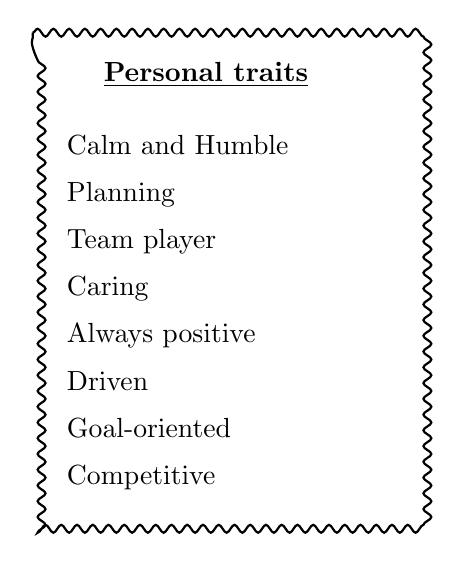
\begin{tikzpicture}
    % Calculate the dimensions of the frame based on the tabular
    \node (table) at (0,0) {
        \begin{tabular}{l}
            \thead{\underline{Personal traits}} \\[10pt]
            \parbox{4cm}{\vspace{0.2cm} 
            Calm and Humble \\[5pt] 
            Planning \\[5pt] 
            Team player \\[5pt] 
            Caring \\[5pt] 
            Always positive \\[5pt] 
            Driven \\[5pt] 
            Goal-oriented \\[5pt] 
            Competitive \vspace{0.2cm}}
        \end{tabular}
    };
    
    % Add a wavy frame around the table
    \draw[thick, decorate, decoration={snake, amplitude=0.5mm, segment length=2mm}]
        ($(table.north west) + (-0.1, 0.1)$) -- ($(table.north east) + (0.1, 0.1)$)
        -- ($(table.south east) + (0.1, -0.1)$) -- ($(table.south west) + (-0.1, -0.1)$)
        -- cycle;
\end{tikzpicture}
\end{minipage}

\section{Other Merits}
\begin{tabularx}{\linewidth}{@{}l X@{}}	
2024 & \textbf{Recipient of multiple scholarships} from \textit{Stiftelsen AAA} and \textit{Anna Whitlocks Minnesfond} following my exchange term \hfill \\[20pt]
2024 & Nominated to an \textbf{exchange term at Nanyang Technological University} \hfill \\[10pt]
2022 & Qualified for membership in \textbf{MENSA} Sweden \hfill \\[10pt]
2019 & \textbf{Driver's license}, B \hfill \\
\end{tabularx}
\nocite{*}
\printbibliography[title={Publications}]
\textit{References/certificates/grades will be provided upon request}.
\vfill
\center{\footnotesize Latest updated: \today \\
CV created in \LaTeX}

\end{document}